\documentclass[12pt, a4paper]{article}
\setlength{\textheight}{24cm}
\setlength{\textwidth}{16cm}
\setlength{\topmargin}{0cm}
\setlength{\evensidemargin}{0cm}
\setlength{\oddsidemargin}{0cm}
\usepackage[affil-it]{authblk}
\usepackage{graphics}
\usepackage{graphicx}
\usepackage{caption}
\usepackage{float}
\usepackage[british]{babel}
\usepackage{hyperref}
\usepackage{subcaption}
\date{}
\begin{document}
\title{Comparison of Some FFT Libraries in C/C++}
\author{Philippe Gambron \thanks{\texttt{philippe.gambron{@}stfc.ac.uk}}, Sue Thorne \thanks{\texttt{sue.thorne{@}stfc.ac.uk}}}
\affil{Science and Technology Facilities Council, Hartree Centre, Rutherford Appleton Laboratory, Harwell Campus, Harwell Oxford, OX11 0QZ, United Kingdom}
\maketitle
\begin{abstract}
We compare the performance of several libraries computing FFTs called from C or C++ code. 
\end{abstract}
\section{Introduction}
Some applications require the computation of the discrete Fourier transform (DFT) of large datasets. In such a case, the efficiency of that step can become of critical importance. In this report, we compare the performance obtained with several libraries that can be called from C or C++.

\section{Benchmark}
The Fourier transform of a discrete signal on a finite domain in one dimension containing $N$ points is given by:
\begin{equation}
{\cal F}_k=\sum_{j=0}^{N-1} x_j e^{-i\frac{2\pi}{N}kj}.
\end{equation}\label{fourier}

We compute it using the Fast Fourier Transform (FFT) method. It consists in expressing the transform recursively as a function of transforms of more sparse subsets of the data. The most famous of these methods is the Cooley-Tukey algorithm \cite{CT}. The procedure can illustrated by rewriting eq. \ref{fourier} and splitting the sum in a part containing the even values of $j$ and another the odd ones, multiplied by a phase factor.
\begin{equation}
{\cal F}_k=\sum_{j=0}^{N/2-1}x_{2j}e^{-i\frac{2\pi}{N}2jk}+e^{-i\frac{2\pi}{N}jk}\sum_{j=0}^{N/2-1}x_{2j+1}e^{-i\frac{2\pi}{n}2jk}
\end{equation}\label{ct}
We can subsequently repeat the procedure by expressing the sums as a function of more sparse transforms till we are left with DFTs of a few data points. This dramatically reduces the number of necessary operations which becomes proportional to $N\log(N)$ rather than $N^2$.\\

We will also consider FFTs in more dimensions. For example, in two dimensions, the discrete transform of complex values $z_{j_x j_y}$ located on a grid consisting of $N_x \times N_y$ points is given by:\\
$$
{\cal F}_{k_x k_y}=\sum_{j_x=0}^{N_x} \sum_{j_y=0}^{N_y} z_{j_x j_y} e^{-i\left(\frac{2\pi}{N_x} j_x k_x+\frac{2\pi}{N_y} j_y k_y\right)}.
$$
The inverse of this transform corresponds to:
$$
{\cal F}_{k_x k_y}=\frac{1}{N_xN_y}\sum_{j_x=0}^{N_x} \sum_{j_y=0}^{N_y} z_{j_x j_y} e^{i\left(\frac{2\pi}{N_x} j_x k_x+\frac{2\pi}{N_y} j_y k_y\right)}.
$$
  


The benchmark \cite{code} consists of calculating the FFT of a series of volumes, in 1, 2 or 3 dimensions, of real or complex values. The purpose was to mimick a problem submitted to us by the CCP PET-MR collaboration \cite{ccppetmr}, within the Software Outlook initiative \cite{softwareoutlook}, who needed to take the transform of a series of square complex images. This example is depicted in Fig. \ref{benchmark} and considered in Section \ref{CCPPETMR}.\\

\begin{figure}[H]
\captionsetup{width=0.6\textwidth}
\centering
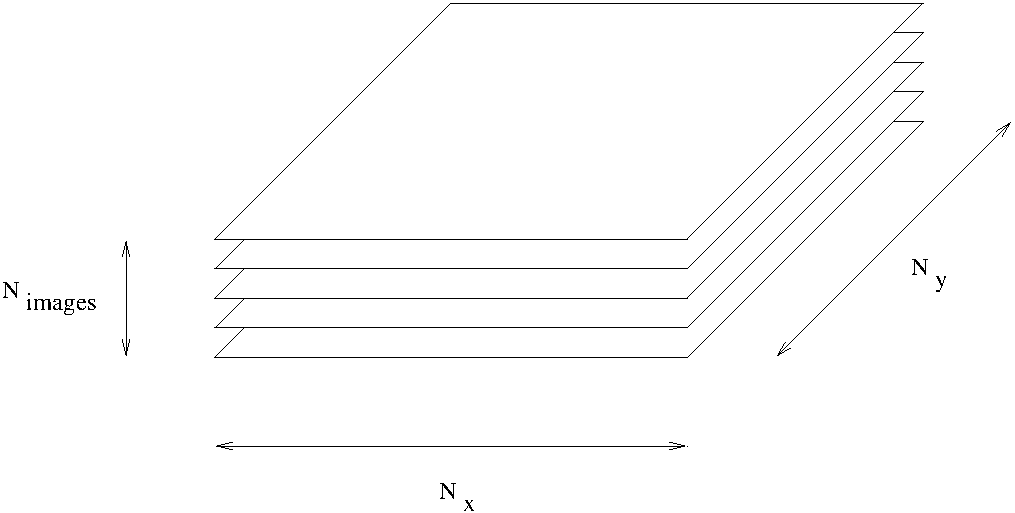
\includegraphics[height=5cm]{benchmark.pdf}
\caption{The benchmark consists in taking the FFT of several images. Each of them is made of real or complex values and can be a simple line, a rectangle or a cuboid.}
\label{benchmark}
\end{figure}

The whole procedure is more precisely depicted in the following pseudocode. We begin by generating \texttt{N\_SIGNALS} signals in 1, 2 or 3 dimensions. These can be real or complex values on a domain of dimensions \texttt{N1}, \texttt{N2}... We then initialise the object performing the FFT and compute the transform. After this step, we repeat the procedure with the inverse transform, in order to compute the error.
\begin{figure}[H]
\captionsetup{width=0.8\linewidth}
\centering
  
\begin{verbatim}
        for i running from 1 to N_SIGNALS
          signal[i]=generate_signal(N_X [,N_Y[, N_Z]])

        initialise FFT

        for i running from 1 to N_SIGNALS
          transform[i]=FFT(signal[i])

        initialise inverse_FFT

        for i running from 1 to N_SIGNALS
          inverse_transform[i]=inverse_FFT(transform[i])

        for i running from 1 to N_SIGNALS
          error=error(||inverse_transform[i]-signal[i]||)
\end{verbatim}
\caption{Pseudocode corresponding to the benchmark}
\label{PSEUDOCODE}
\end{figure}

We used a number of points varying from $\sim 10^3$ to $\sim 10^7$ in 1, 2 and 3 dimensions. The domains had sides of equal lengths (square or cubic) or were flattened (rectangle or cuboid). These dimensions could be powers of 2, products of powers of small integers or prime numbers\\

The values appearing in the graphs are the execution time averaged over 10 runs. A certain number of bumps or slight unexpected features are apparent. However they were consistently repeated in all our measurements. This is also confirmed by the standard deviation of our results which was always quite small, of the order of a few percents of the average value. We chose not to display error bars on our graphs since they were so small that they were barely visible. 

\section{Overview of the chosen libraries}
We consider the following libraries computing FFTs: FFTW \cite{fftw}, MKL \cite{mkl}, GSL \cite{gsl} and FFTPACK \cite{fftpack} (Table \ref{ffttable}). They can perform complex transforms, real-to-half-complex ones (and conversely) as well as, in the case of FFTW, real-to-real transforms when the signal is odd or even. The half-complex output consists in half as many complex values as there were points in the signal, taking advantage of the hermiticity of the Fourier transform of a real function.\\

The GSL and FFTPACK libraries only work in one dimension\footnote{FFTPACK can compute FFTs in several dimensions but it is written in FORTRAN and all the C or C++ wrappers we have found only allowed one-dimensional transforms.}. On the contrary, FFTW and MKL can compute FFTs in several dimensions. They are also capable of working in a parallel way, using multithreading and MPI.  
\begin{table}[H]
\captionsetup{width=1\textwidth}
\begin{tabular}{|p{2.5cm}||p{2.5cm}|p{1cm}|p{3cm}|p{3cm}|p{2cm}|p{2cm}|}
\hline
& Type & Dim. & Radices & Parallelism & Licence \\
\hline
\hline
FFTW & R$\to$H,\ \ \  C$\to$C,\ \ \  H$\to$R, R{\scriptsize (odd/even)}$\to$R& Any&2, 3, 5, 7, 11, 13 + any with code generator & Multithreading, MPI & GPL v2\\
\hline
MKL  &  R$\to$H,\ \ \  C$\to$C,\ \ \ \  H$\to$R& Any & & Multithreading, MPI & Proprietary\\
\hline
GSL  &  R$\to$H,\ \ \  C$\to$C,\ \ \ \  H$\to$R & 1 & 2, 3, 5, 6, 7 & - & GPL v3\\
\hline
FFTPACK {\scriptsize (CASA wrapper)} &  R$\to$H,\ \ \  C$\to$C,\ \ \ \  H$\to$R & 1 & & - & GPL v2\\
\hline
\end{tabular}
\caption{Overview of the FFT libraries considered. R stands for real, C, for complex, and HC, for half-complex.}
\label{ffttable}
\end{table}

\section{Set up}
Our measurements were carried out on ARCHER \cite{archer}, the UK National Supercomputing Service. It is made of 4920 compute nodes each containing  two 12-core Intel E5-2697 v2 (Ivy Bridge) processors and at least 64 GB of RAM. The modules \texttt{gcc/7.2.0} and \\ \texttt{intel/17.0.3.191} were loaded. In order to take advantage of multi-threading, the environment variable \texttt{KMP\_AFFINITY} must be set to \texttt{disabled}.\\

Our benchmark was coded in C++ using double-precision reals. More precisely, we used version 3.3.8 of FFTW, version 17.0.3 of MKL and version 2.5 of GSL. Note that we used our own version of Boost, FFTW and GSL because the version of Boost present on the system was lacking certain libraries and we wanted to use the most recent versions of FFTW and GSL. The benchmark was compiled with the flags \texttt{-std=c++1z -O3  -fopenmp   -lm -lfftw3 -lfftw3\_threads -lgslcblas -lgsl -lboost\_system -lboost\_chrono -liomp5 -lmkl\_core -lmkl\_intel\_thread \\-lmkl\_intel\_lp64  -lcasa\_scimath  -llapack}.\\

Since FFTPACK was written in FORTRAN, we have resorted to the C++ wrapper provided by CASA, the radioastronomy package \cite{casa}. This is straightforward to install on Debian-like systems, as the one used by CCP PET-MR in their virtual environment, where CASA can be installed using the package manager. However, including the headers and linking with the libraries was not possible with the version of CASA distributed by the National Radio Astronomy Observatory. As a consequence, this was quite difficult to set up on ARCHER and required the use of libraries provided by an old version of Debian to match those available on the system. For this reason, it was necessary to use as well an older version of CASA, 2.4.0.

\pagebreak
\section{Effect of the domain size in one dimension}\label{PERFORMANCE1D}

In this section, we compare the performance of each library, in one dimension, for numbers of points consisting of powers of 2, products of powers of small integers and prime numbers. We do so for real and complex values and with FFTW (Fig. \ref{1DFFTWR} and \ref{1DFFTWC}), MKL (Fig. \ref{1DMKLR} and \ref{1DMKLC}), GSL (Fig. \ref{1DGSLR} and \ref{1DGSLC}) and FFTPACK (Fig. \ref{1DFFTPACKR} and \ref{1DFFTPACKC}). We then compare the different libraries for powers of 2 (Fig. \ref{1DPOW2R} and \ref{1DPOW2C}) and in general (Fig. \ref{1DR} and \ref{1DC}).\\

Our example corresponds to the pseudocode in Table \ref{PSEUDOCODE}. In this case, we use a single signal and the number of points is a power of 2, an integer number of the form $2^j3^k5^l7^m$ or a prime number, both close to the corresponding power of 2.
\begin{table}[H]
\centering
\begin{tabular}{|l|l|l|}
  \hline
  \multicolumn{3}{|c|}{$N$}\\
  \hline
  \hline
Powers of 2 & product of integers & primes\\ \hline
$2^8=256$	 & $2^2\ 3^2\ 5\ 7=210$	     & 257  \\ \hline
$2^{10}=1024$	 & $2^2\ 3^2\ 5\ 7=1260$	     & 1021  \\ \hline
$2^{12}=4096$	 & $2\ 3^2\ 5\ 7=4410$	     & 4093 \\ \hline
$2^{14}=16384$	 & $2\ 3^2\ 5^3\ 7=15750$	     & 16381 \\ \hline
$2^{16}=65536$	 & $2\ 3^3\ 5^2\ 7^2=66150$      & 65521 \\ \hline
$2^{18}=262144$	 & $2\ 3\ 5^3\ 7^3=257250$       & 262139 \\ \hline
$2^{20}=1048576$  & $2\ 3^2\ 5^2\ 7^4=1080450$    & 1048573 \\ \hline
$2^{22}=4194304$  & $2^2\ 3^2\ 5^2 7^4=4321800$  &	\\ \hline
$2^{24}=16777216$ & $2^3\ 3^2\ 5^4\ 7^3=15435000$ &	\\ \hline
$2^{26}=67108864$ & $2^3\ 3^3\ 5^3\ 7^4=64827000$ &\\ \hline
\end{tabular}
\caption{Number of points used for the benchmark in one dimension}
\end{table}



We begin by comparing the performance obtained with powers of 2, products of small integers and primes. As expected, for all the libraries, the performance is worse with primes than in the other cases. 
\begin{figure}[H]
\captionsetup{width=0.8\linewidth}
\centering
\begin{subfigure}{.5\textwidth}
\centering
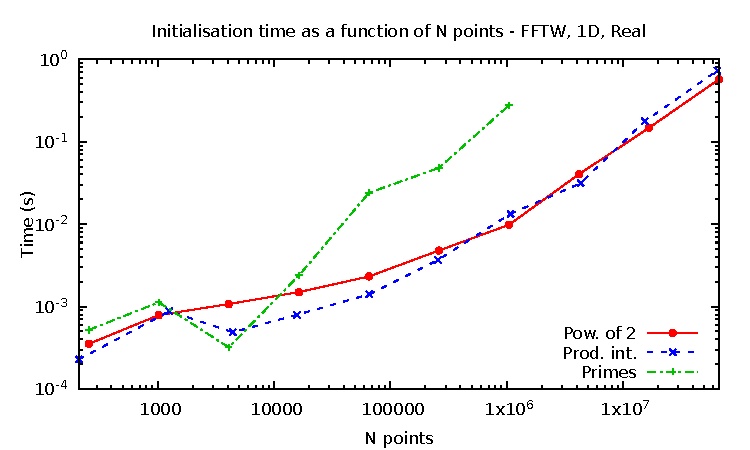
\includegraphics[width=.9\linewidth]{graphs/1d-fftw-init-r.pdf}
\caption{Intialisation (real)}
\label{1DFFTWRI}
\end{subfigure}%
\begin{subfigure}{.5\textwidth}
\centering
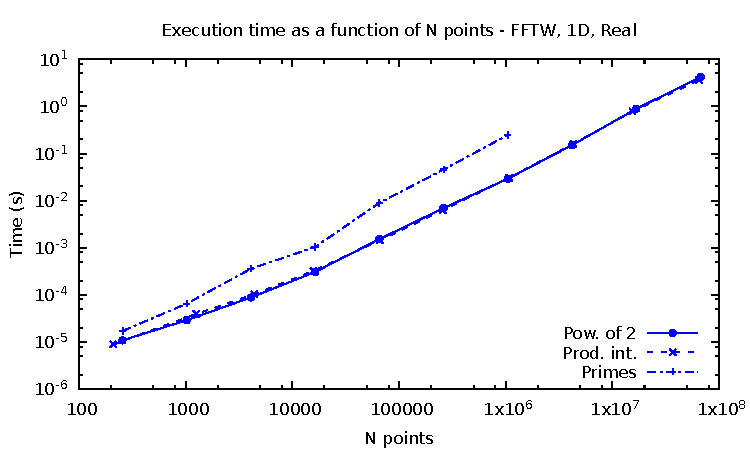
\includegraphics[width=.9\linewidth]{graphs/1d-fftw-exec-r.pdf}
\caption{Execution (real)}
\label{1DFFTWR}
\end{subfigure}\\
\begin{subfigure}{.5\textwidth}
\centering
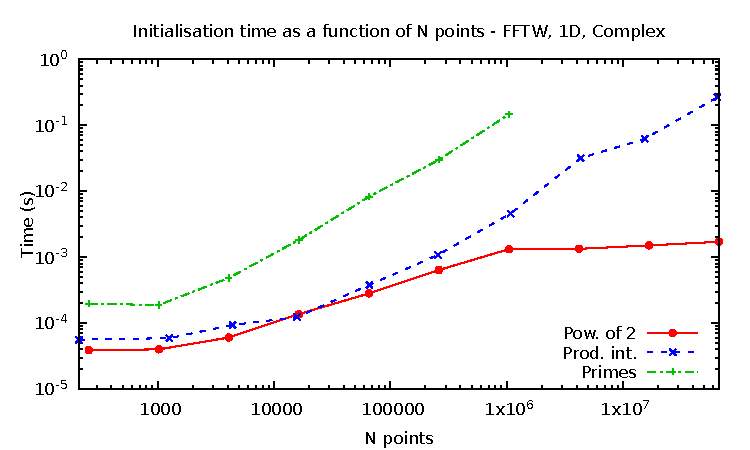
\includegraphics[width=.9\linewidth]{graphs/1d-fftw-init-c.pdf}
\caption{Intialisation (complex)}
\label{1DFFTWCI}
\end{subfigure}%
\begin{subfigure}{.5\textwidth}
\centering
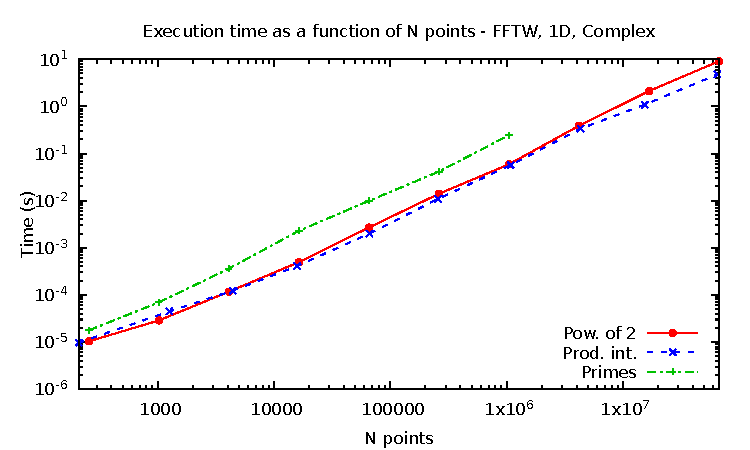
\includegraphics[width=.9\linewidth]{graphs/1d-fftw-exec-c.pdf}
\caption{Execution (complex)}
\label{1DFFTWC}
\end{subfigure}
\caption{Initialisation and execution times as a function of the number of points (1 dimension, FFTW, 1 thread)}
\label{1DFFTW}
\end{figure}

\begin{figure}[H]
\captionsetup{width=0.8\linewidth}
\centering
\begin{subfigure}{.5\textwidth}
\centering
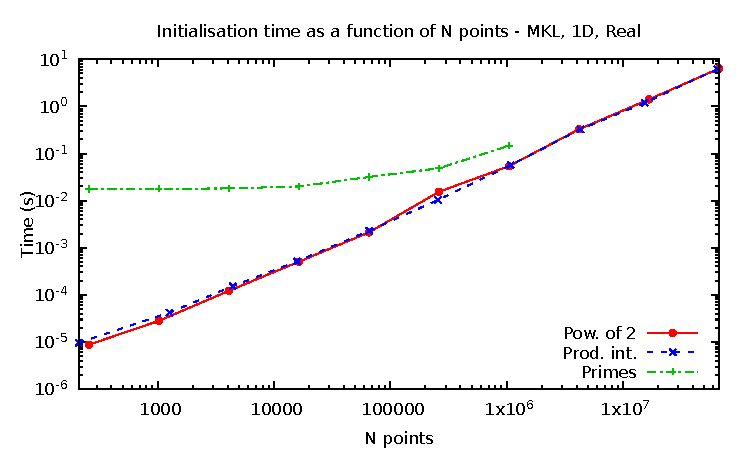
\includegraphics[width=.9\linewidth]{graphs/1d-mkl-init-r.pdf}
\caption{Intialisation (real)}
\label{1DMKLRI}
\end{subfigure}%
\begin{subfigure}{.5\textwidth}
\centering
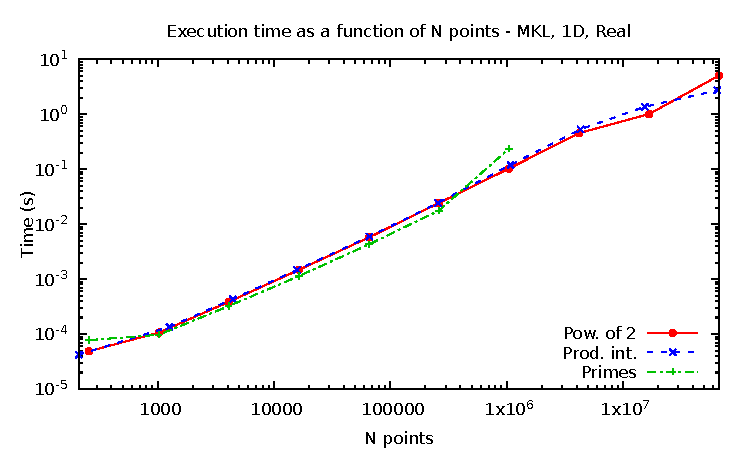
\includegraphics[width=.9\linewidth]{graphs/1d-mkl-exec-r.pdf}
\caption{Execution (real)}
\label{1DMKLR}
\end{subfigure}\\
\begin{subfigure}{.5\textwidth}
\centering
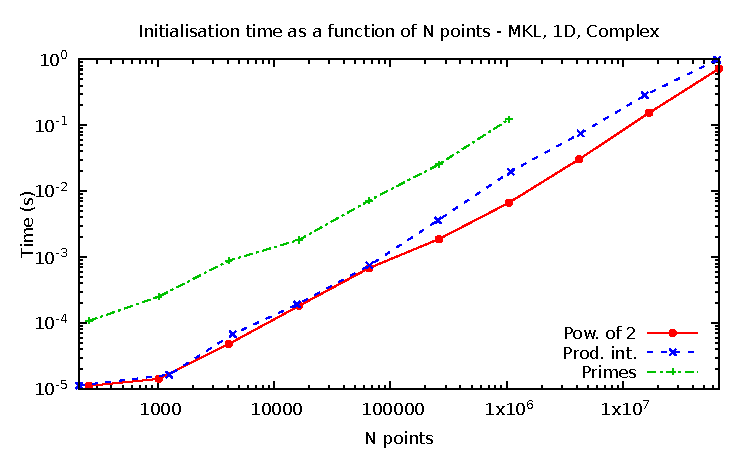
\includegraphics[width=.9\linewidth]{graphs/1d-mkl-init-c.pdf}
\caption{Intialisation (complex)}
\label{1DMKLCI}
\end{subfigure}%
\begin{subfigure}{.5\textwidth}
\centering
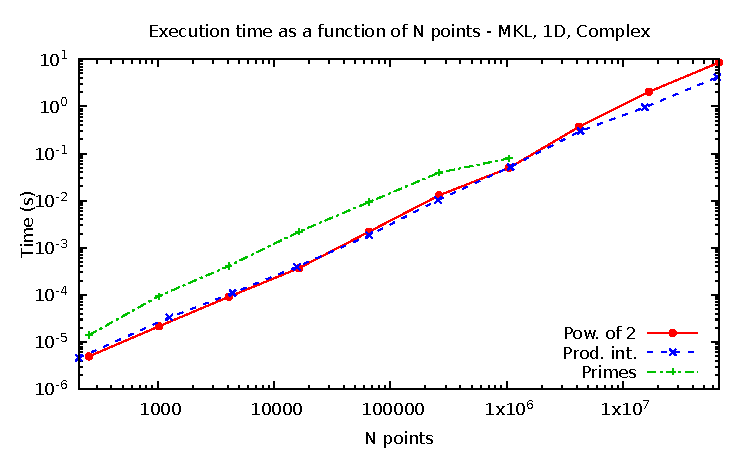
\includegraphics[width=.9\linewidth]{graphs/1d-mkl-exec-c.pdf}
\caption{Execution (complex)}
\label{1DMKLC}
\end{subfigure}\\
\caption{Initialisation and execution times as a function of the number of points (1 dimension, MKL, 1 thread)}
\label{1DMKL}
\end{figure}

\begin{figure}[H]
\captionsetup{width=0.8\linewidth}
\centering
\begin{subfigure}{.5\textwidth}
\centering
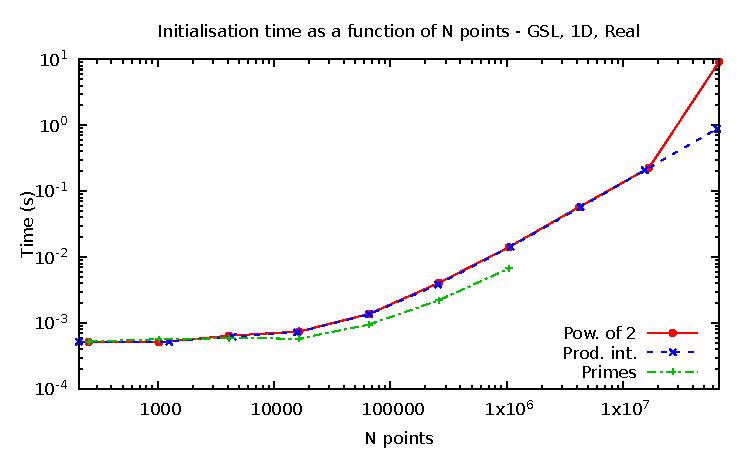
\includegraphics[width=.9\linewidth]{graphs/1d-gsl-init-r.pdf}
\caption{Intialisation (real)}
\label{1DGSLRI}
\end{subfigure}%
\begin{subfigure}{.5\textwidth}
\centering
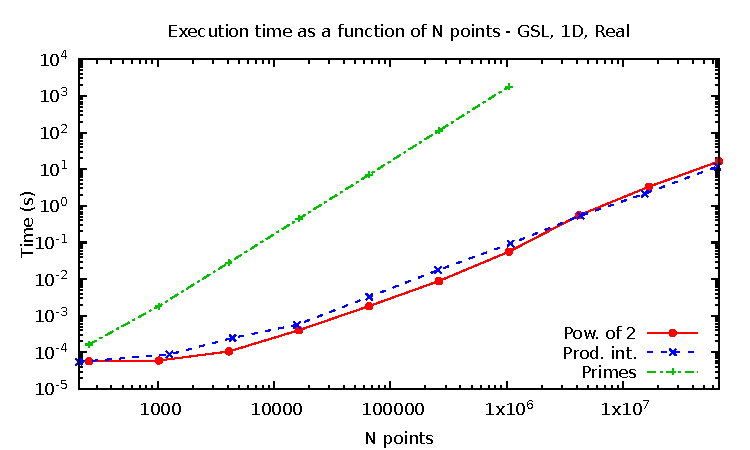
\includegraphics[width=.9\linewidth]{graphs/1d-gsl-exec-r.pdf}
\caption{Execution (real)}
\label{1DGSLR}
\end{subfigure}\\
\begin{subfigure}{.5\textwidth}
\centering
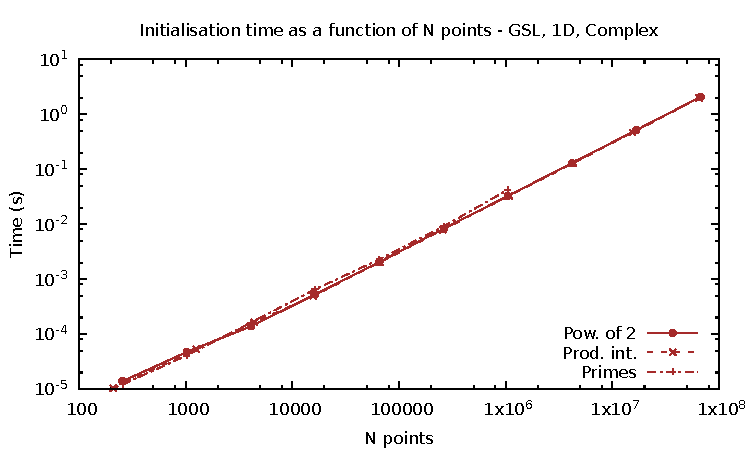
\includegraphics[width=.9\linewidth]{graphs/1d-gsl-init-c.pdf}
\caption{Intialisation (complex)}
\label{1DGSLCI}
\end{subfigure}%
\begin{subfigure}{.5\textwidth}
\centering
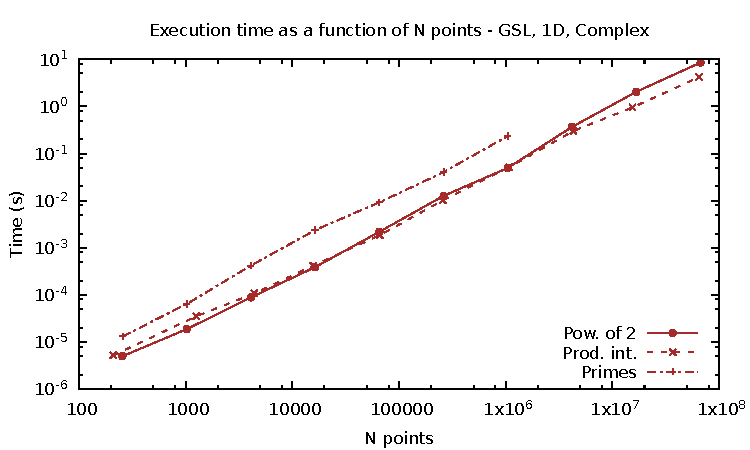
\includegraphics[width=.9\linewidth]{graphs/1d-gsl-exec-c.pdf}
\caption{Execution (complex)}
\label{1DGSLC}
\end{subfigure}
\caption{Initialisation and execution times as a function of the number of points (1 dimension, GSL, 1 thread)}
\label{1DGSL}
\end{figure}

\begin{figure}[H]
\captionsetup{width=0.8\linewidth}
\centering
\begin{subfigure}{.5\textwidth}
\centering
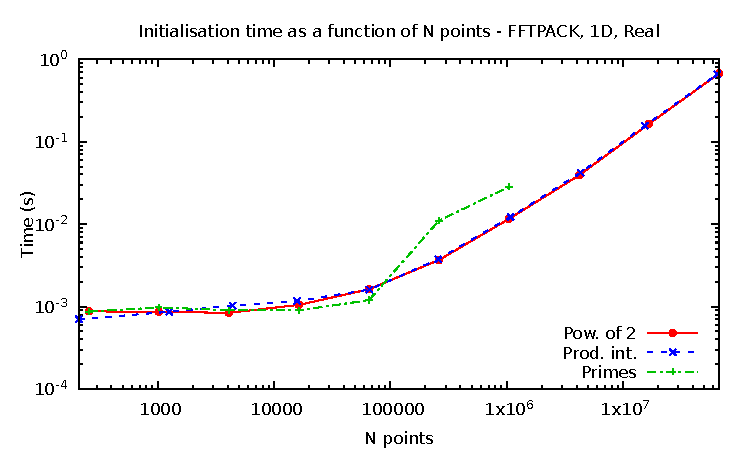
\includegraphics[width=.9\linewidth]{graphs/1d-fftpack-init-r.pdf}
\caption{Intialisation (real)}
\label{1DFFTPACKRI}
\end{subfigure}%
\begin{subfigure}{.5\textwidth}
\centering
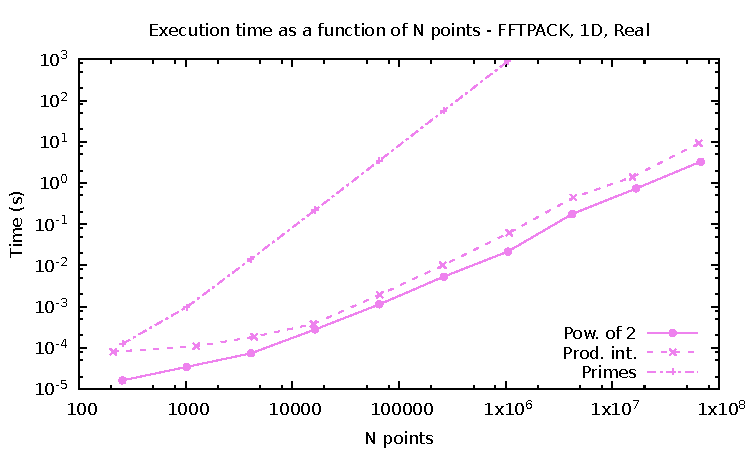
\includegraphics[width=.9\linewidth]{graphs/1d-fftpack-exec-r.pdf}
\caption{Execution (real)}
\label{1DFFTPACKR}
\end{subfigure}\\
\begin{subfigure}{.5\textwidth}
\centering
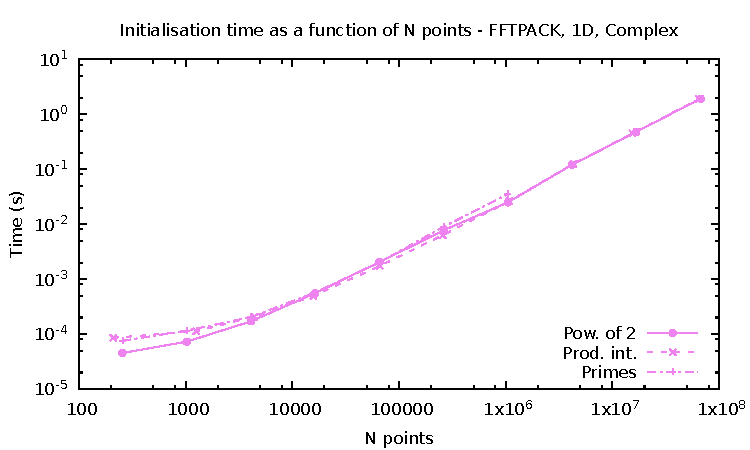
\includegraphics[width=.9\linewidth]{graphs/1d-fftpack-init-c.pdf}
\caption{Intialisation (complex)}
\label{1DFFTPACKCI}
\end{subfigure}%
\begin{subfigure}{.5\textwidth}
\centering
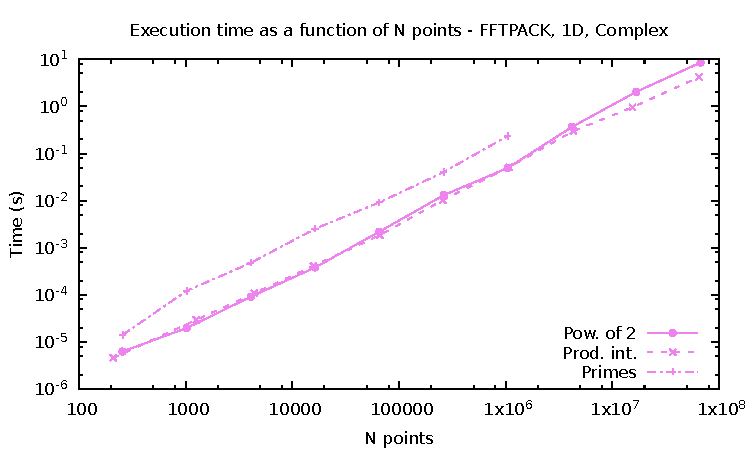
\includegraphics[width=.9\linewidth]{graphs/1d-fftpack-exec-c.pdf}
\caption{Execution (complex)}
\label{1DFFTPACKC}
\end{subfigure}
\caption{Initialisation and execution times as a function of the number of points (1 dimension, FFTPACK, 1 thread)}
\label{1DFFTPACK}
\end{figure}

We also compared the libraries among themselves for powers of 2 (Table \ref{1DPOW2}) and in general (Table \ref{1D}).  According ot our measurements, the MKL library tends to be the fastest. We also notice that the performance with primes is significantly worse, with real numbers, in the cases of GSL and FFTPACK.

\begin{figure}[H]
\captionsetup{width=0.8\linewidth}
\centering
\begin{subfigure}{.5\textwidth}
\centering
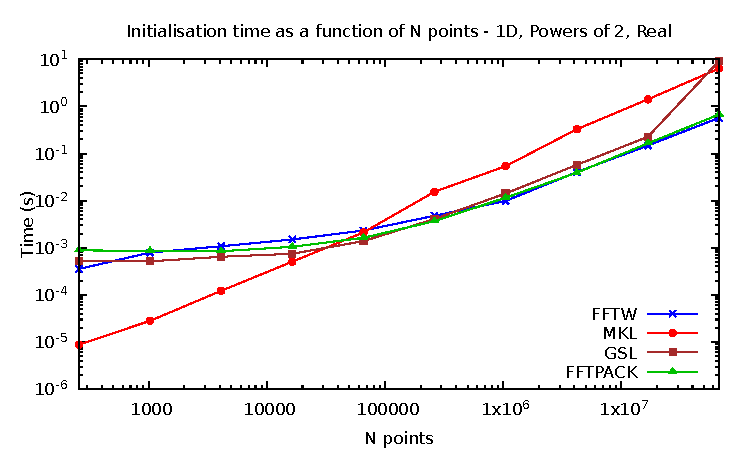
\includegraphics[width=.9\linewidth]{graphs/1d-pow2-init-r.pdf}
\caption{Intialisation (real)}
\label{1DPOW2RI}
\end{subfigure}%
\begin{subfigure}{.5\textwidth}
\centering
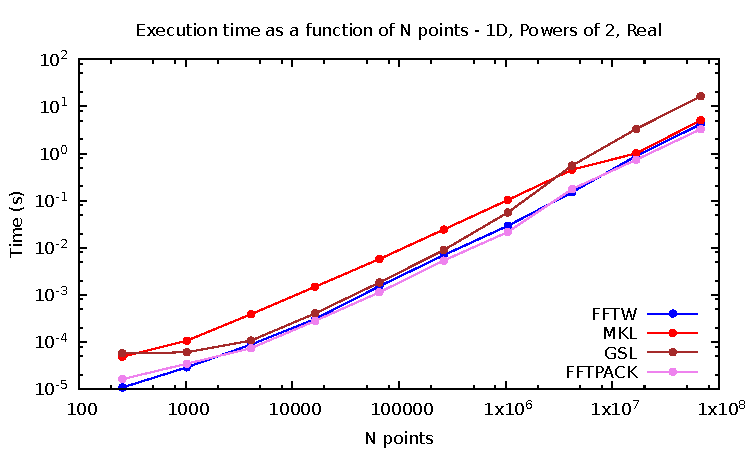
\includegraphics[width=.9\linewidth]{graphs/1d-pow2-exec-r.pdf}
\caption{Execution (real)}
\label{1DPOW2R}
\end{subfigure}\\
\begin{subfigure}{.5\textwidth}
\centering
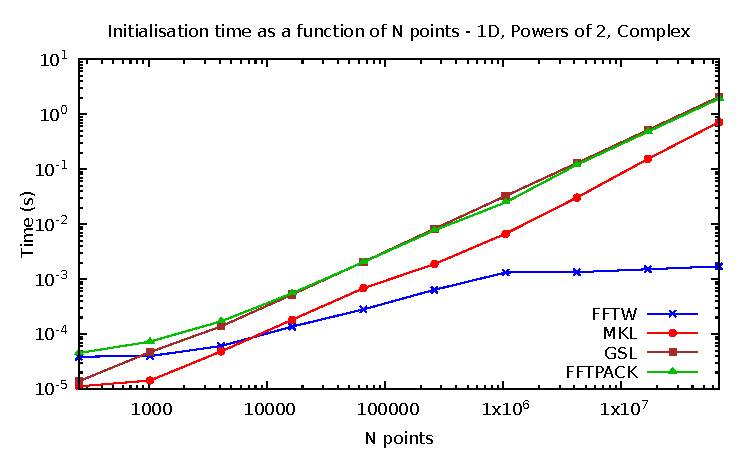
\includegraphics[width=.9\linewidth]{graphs/1d-pow2-init-c.pdf}
\caption{Intialisation (complex)}
\label{1DPOW2CI}
\end{subfigure}%
\begin{subfigure}{.5\textwidth}
\centering
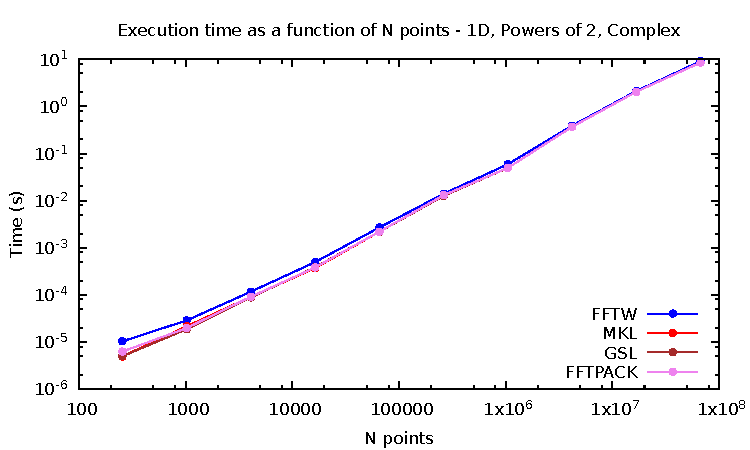
\includegraphics[width=.9\linewidth]{graphs/1d-pow2-exec-c.pdf}
\caption{Execution (complex)}
\label{1DPOW2C}
\end{subfigure}
\caption{Initialisation and execution times as a function of the number of points (1 dimension, powers of 2, 1 thread)}
\label{1DPOW2}
\end{figure}

\begin{figure}[H]
\captionsetup{width=0.8\linewidth}
\centering
\begin{subfigure}{.5\textwidth}
\centering
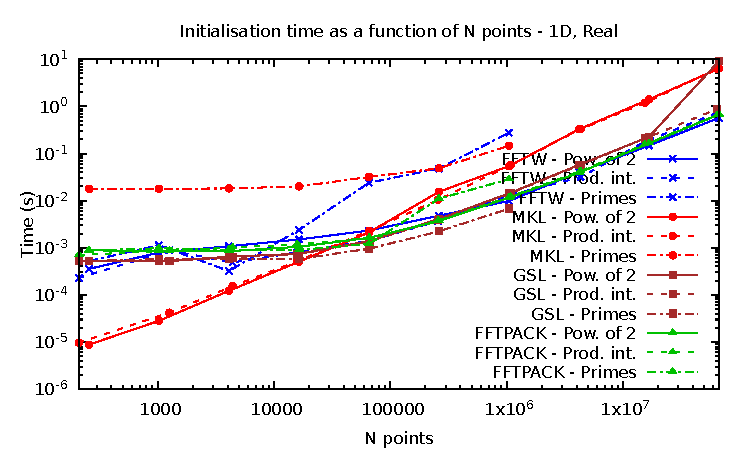
\includegraphics[width=.9\linewidth]{graphs/1d-init-r.pdf}
\caption{Intialisation (real)}
\label{1DRI}
\end{subfigure}%
\begin{subfigure}{.5\textwidth}
\centering
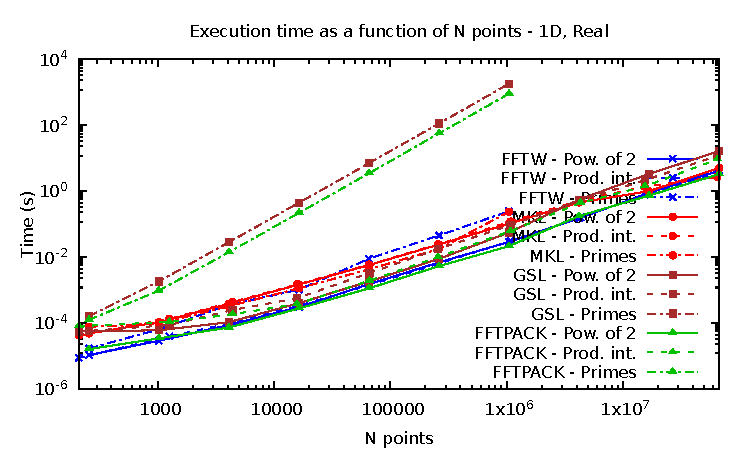
\includegraphics[width=.9\linewidth]{graphs/1d-exec-r.pdf}
\caption{Execution (real)}
\label{1DR}
\end{subfigure}\\
\begin{subfigure}{.5\textwidth}
\centering
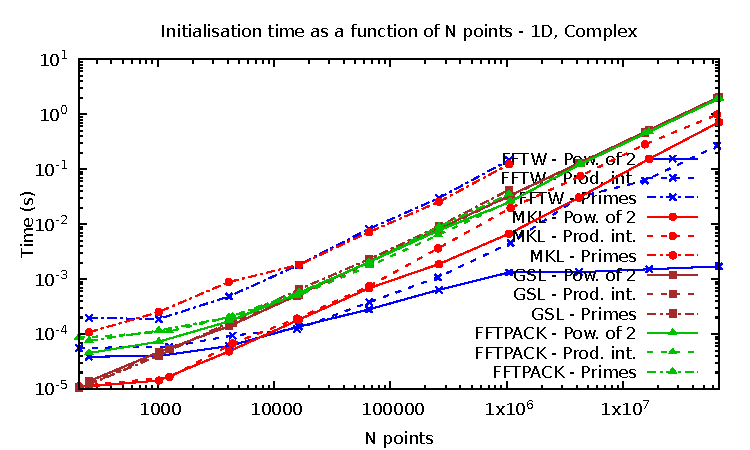
\includegraphics[width=.9\linewidth]{graphs/1d-init-c.pdf}
\caption{Intialisation (complex)}
\label{1DCI}
\end{subfigure}%
\begin{subfigure}{.5\textwidth}
\centering
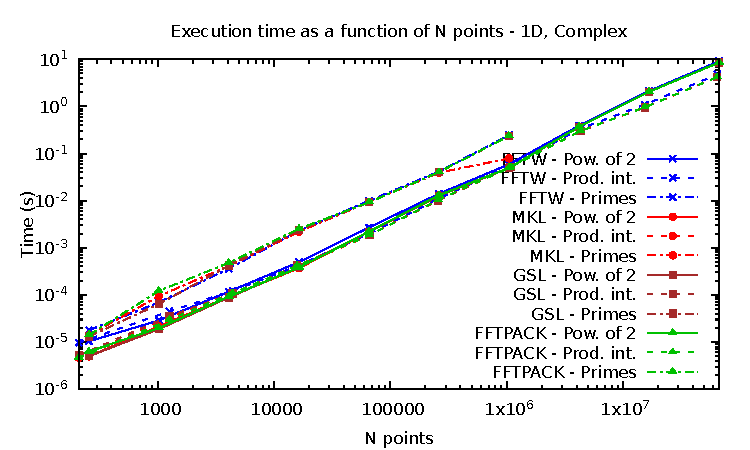
\includegraphics[width=.9\linewidth]{graphs/1d-exec-c.pdf}
\caption{Execution (complex)}
\label{1DC}
\end{subfigure}
\caption{Initialisation and execution times as a function of the number of points (1 dimension, 1 thread)}
\label{1D}
\end{figure}

\section{Effect of the domain size for 2D problems}\label{PERFORMANCE2D}

In this section, we measure the performance obtained in two dimensions, on a square domain. However, only FFTW and MKL work in these situations (Fig. \ref{2DFFTWR} - \ref{3DC}).\\

We begin by comparing the performance obtained, for a single signal, with numbers of points that are a power of 2, the product of small integers or a prime number. These numbers are chosen as in Section \ref{PERFORMANCE1D} and we endeavoured make the total number of points vary with a similar range. The dimensions we chose appear in the following table.\\

\begin{table}[H]
\centering
\begin{tabular}{|l|l|l|}
  \hline
  \multicolumn{3}{|c|}{$N_x=N_y$}\\
  \hline
  \hline
Powers of 2 & prod. of int. & primes\\ \hline
$2^9=512$ & $2^3\ 3^2\ 7=504$ & 509\\ \hline
$2^{10}=1024$ & $3\ 7^3=1029$ & 1021\\ \hline
$2^{11}=2048$ & $2\ 3\ 7^3=2058$ & 2027\\ \hline
$2^{12}=4096$ & $2^2\ 3\ 7^3=4116$ & 4049\\ \hline
$2^{13}=8192$ & $2^3\ 3\ 7^3=8232$ & 8123\\ \hline
\end{tabular}
\caption{Number of points used for the benchmark in two dimensions}
\end{table}


 As in one dimension (Section \ref{PERFORMANCE1D}), we obtain the best performance when the number of elements on each side is a power of 2 or the product of small integers rather than a prime number. We also observe that the MKL library tends to be the most efficient as well in 2 dimensions.
 

\begin{figure}[H]
\captionsetup{width=0.8\linewidth}
\centering
\begin{subfigure}{.5\textwidth}
\centering
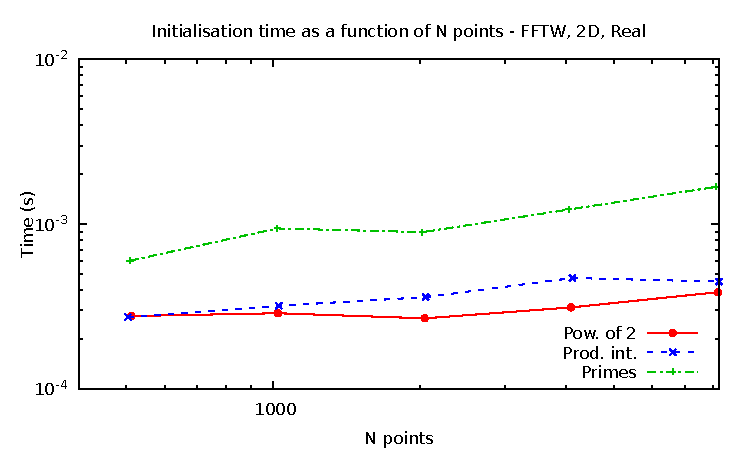
\includegraphics[width=.9\linewidth]{graphs/2d-fftw-init-r.pdf}
\caption{Intialisation (real)}
\label{2DFFTWRI}
\end{subfigure}%
\begin{subfigure}{.5\textwidth}
\centering
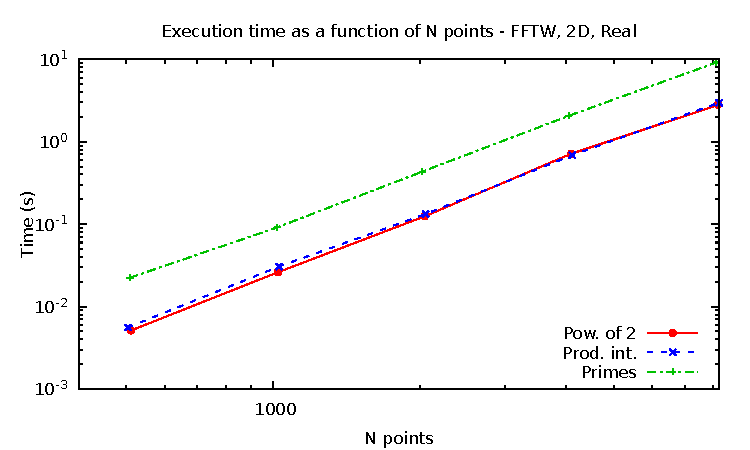
\includegraphics[width=.9\linewidth]{graphs/2d-fftw-exec-r.pdf}
\caption{Execution (real)}
\label{2DFFTWR}
\end{subfigure}\\
\begin{subfigure}{.5\textwidth}
\centering
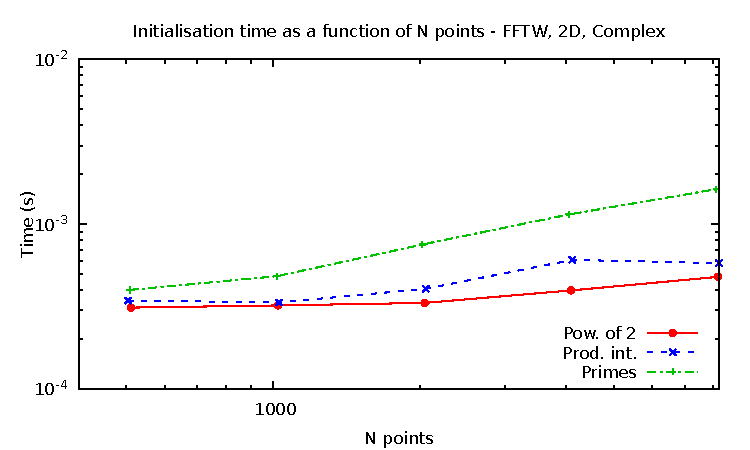
\includegraphics[width=.9\linewidth]{graphs/2d-fftw-init-c.pdf}
\caption{Intialisation (complex)}
\label{2DFFTWCI}
\end{subfigure}%
\begin{subfigure}{.5\textwidth}
\centering
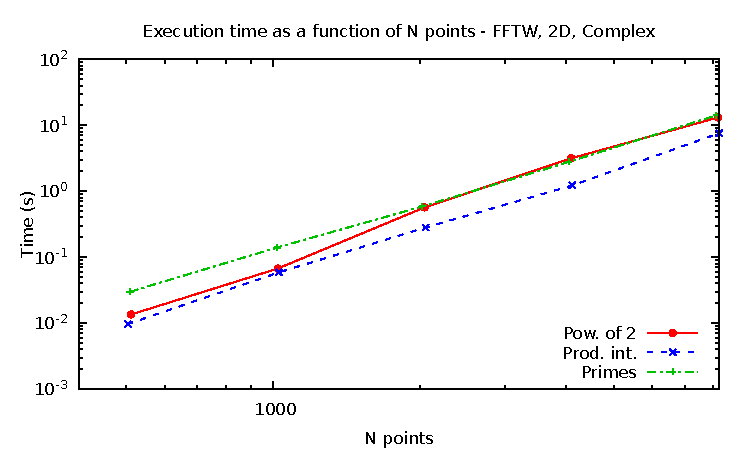
\includegraphics[width=.9\linewidth]{graphs/2d-fftw-exec-c.pdf}
\caption{Execution (complex)}
\label{2DFFTWC}
\end{subfigure}
\caption{Initialisation and execution times as a function of square side (2 dimensions, FFTW, 1 thread)}
\label{2DFFTW}
\end{figure}
\begin{figure}[H]
\captionsetup{width=0.8\linewidth}
\centering
\begin{subfigure}{.5\textwidth}
\centering
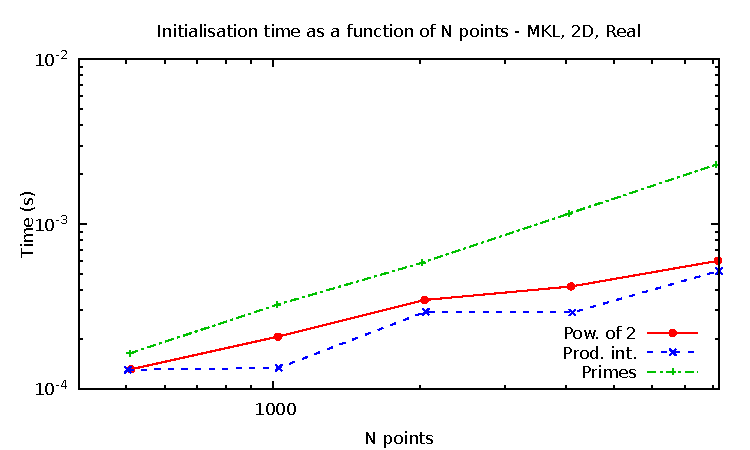
\includegraphics[width=.9\linewidth]{graphs/2d-mkl-init-r.pdf}
\caption{Intialisation (real)}
\label{2DMKLRI}
\end{subfigure}%
\begin{subfigure}{.5\textwidth}
\centering
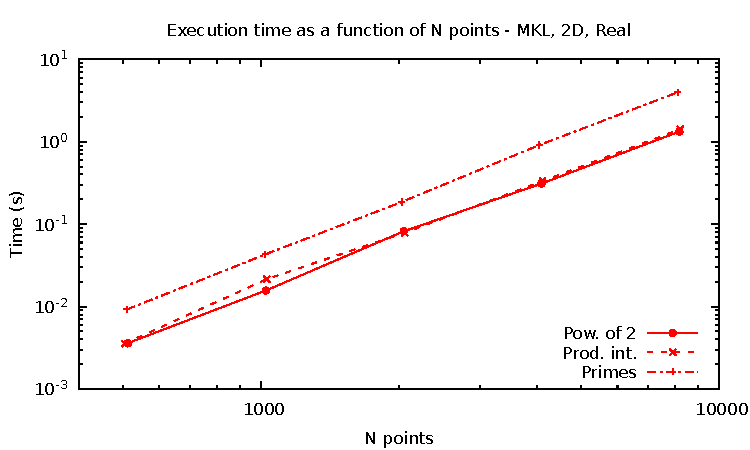
\includegraphics[width=.9\linewidth]{graphs/2d-mkl-exec-r.pdf}
\caption{Execution (real)}
\label{2DMKLR}
\end{subfigure}\\
\begin{subfigure}{.5\textwidth}
\centering
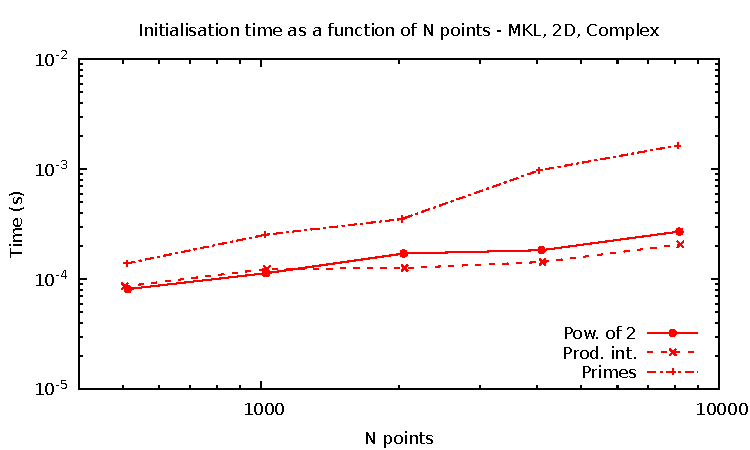
\includegraphics[width=.9\linewidth]{graphs/2d-mkl-init-c.pdf}
\caption{Intialisation (complex)}
\label{2DMKLCI}
\end{subfigure}%
\begin{subfigure}{.5\textwidth}
\centering
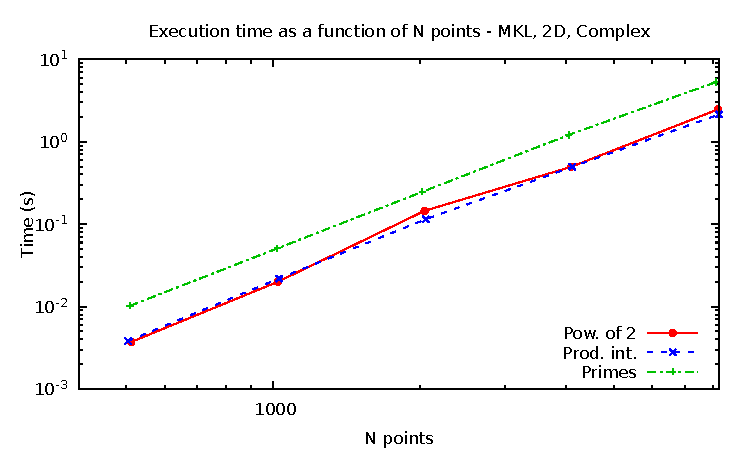
\includegraphics[width=.9\linewidth]{graphs/2d-mkl-exec-c.pdf}
\caption{Execution (complex)}
\label{2DMKLC}
\end{subfigure}
\caption{Initialisation and execution times as a function of square side (2 dimensions, MKL, 1 thread)}
\label{2DMKL}
\end{figure}

\begin{figure}[H]
\captionsetup{width=0.8\linewidth}
\centering
\begin{subfigure}{.5\textwidth}
\centering
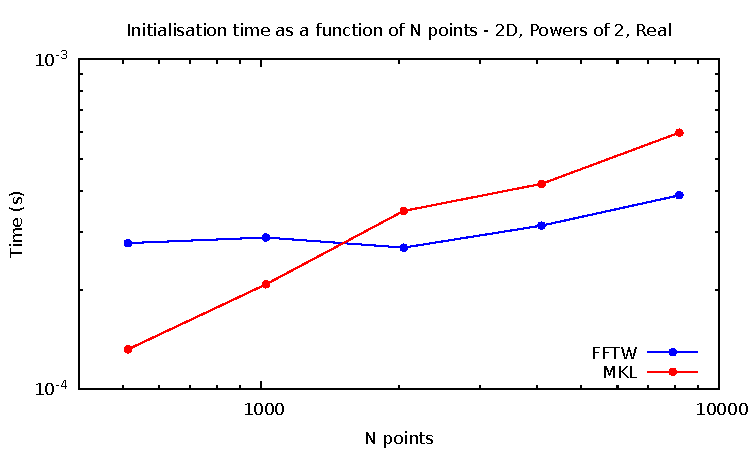
\includegraphics[width=.9\linewidth]{graphs/2d-pow2-init-r.pdf}
\caption{Intialisation (real)}
\label{2DPOW2RI}
\end{subfigure}%
\begin{subfigure}{.5\textwidth}
\centering
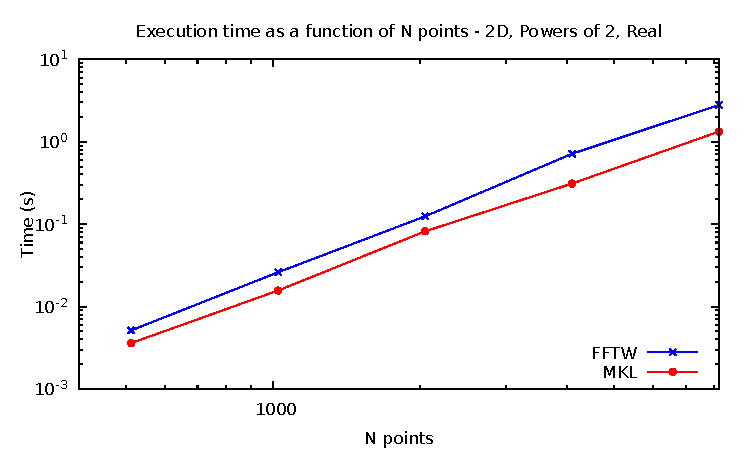
\includegraphics[width=.9\linewidth]{graphs/2d-pow2-exec-r.pdf}
\caption{Execution (real)}
\label{2DPOW2R}
\end{subfigure}\\
\begin{subfigure}{.5\textwidth}
\centering
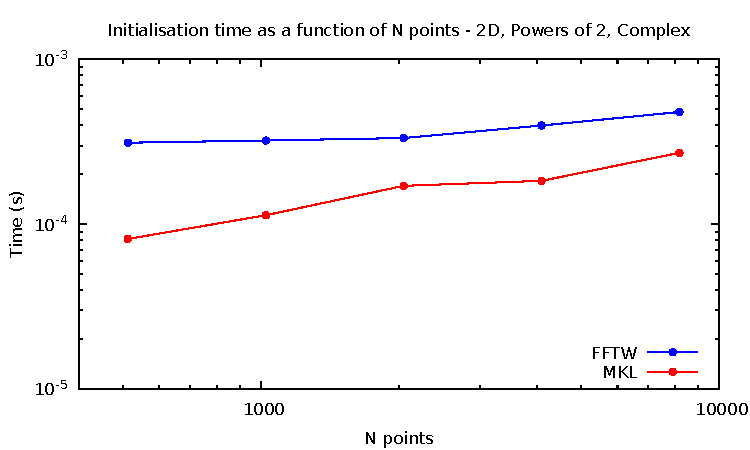
\includegraphics[width=.9\linewidth]{graphs/2d-pow2-init-c.pdf}
\caption{Intialisation (complex)}
\label{2DPOW2CI}
\end{subfigure}%
\begin{subfigure}{.5\textwidth}
\centering
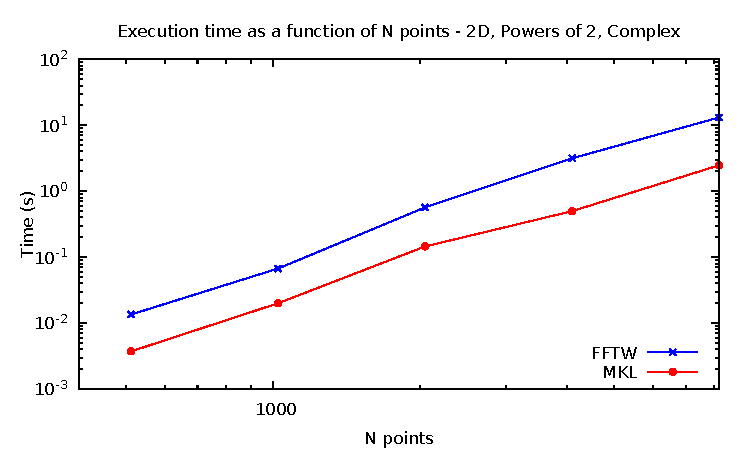
\includegraphics[width=.9\linewidth]{graphs/2d-pow2-exec-c.pdf}
\caption{Execution (complex)}
\label{2DPOW2C}
\end{subfigure}
\caption{Initialisation and execution times as a function of square side (2 dimensions, powers of 2, 1 thread)}
\label{2DPOW2}
\end{figure}


\begin{figure}[H]
\captionsetup{width=0.8\linewidth}
\centering
\begin{subfigure}{.5\textwidth}
\centering
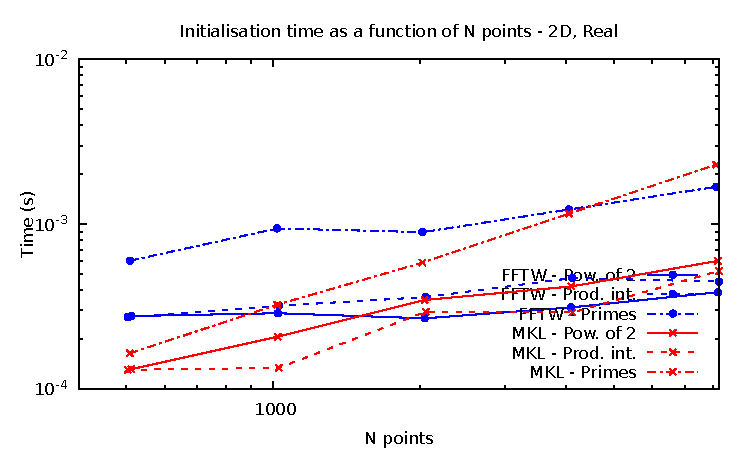
\includegraphics[width=.9\linewidth]{graphs/2d-init-r.pdf}
\caption{Intialisation (real)}
\label{2DRI}
\end{subfigure}%
\begin{subfigure}{.5\textwidth}
\centering
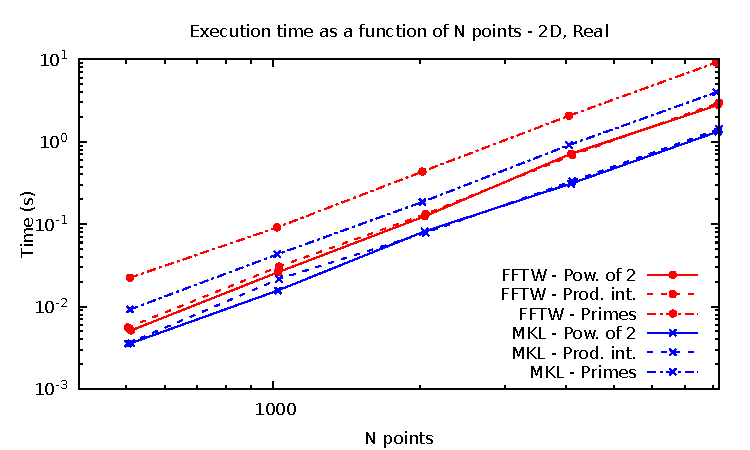
\includegraphics[width=.9\linewidth]{graphs/2d-exec-r.pdf}
\caption{Execution (real)}
\label{2DR}
\end{subfigure}\\
\begin{subfigure}{.5\textwidth}
\centering
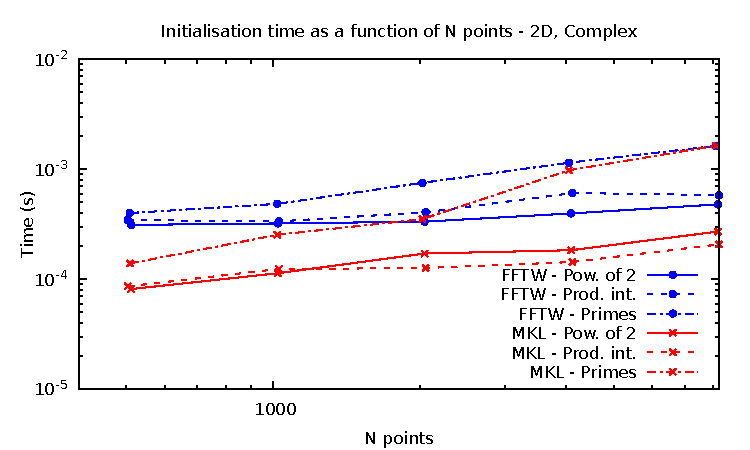
\includegraphics[width=.9\linewidth]{graphs/2d-init-c.pdf}
\caption{Intialisation (complex)}
\label{2DCI}
\end{subfigure}%
\begin{subfigure}{.5\textwidth}
\centering
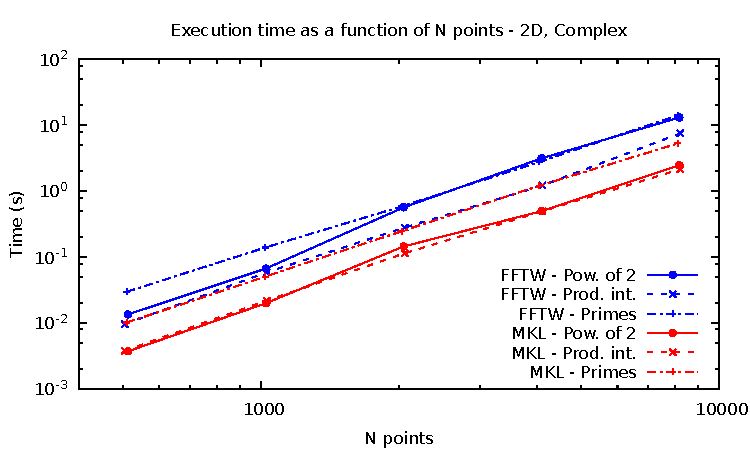
\includegraphics[width=.9\linewidth]{graphs/2d-exec-c.pdf}
\caption{Execution (complex)}
\label{2DC}
\end{subfigure}
\caption{Initialisation and execution times as a function of square side (2 dimensions, 1 thread)}
\label{2D}
\end{figure}

\section{Effect of the domain size for 3D problems}\label{PERFORMANCE3D}

We repeat the analysis carried out in Sections \ref{PERFORMANCE1D} and \ref{PERFORMANCE2D} in three dimensions, on a cubic domain, with  the FFTW and MKL libraries. In this case, the number of points is given in the following table.\\

\begin{table}[H]
\centering
\begin{tabular}{|l|l|l|}
  \hline
  \multicolumn{3}{|c|}{$N_x=N_y=N_z$}\\
  \hline
  \hline
  Powers of 2 & prod. of int. & primes\\ \hline
$2^5=32$ & $2\ 3\ 5=30$	& 31\\ \hline
$2^6=64$ & $2\ 5\ 7=70$	& 61\\ \hline
$2^7=128$ & $3\ 5\ 7=105$ & 127\\ \hline
$2^8=256$ & $2\ 3\ 5\ 7=210$ & 257\\ \hline
$2^9=512$ & $2^2\ 3\ 5\ 7=420$ & 509\\ \hline
\end{tabular}
\caption{Number of points used for the benchmark in three dimensions}
\end{table}

As previously, the best performance is achieved when the number of points is a power of 2 or the product of small integers rather than a prime number. We also observe that the MKL library is more efficient.
\begin{figure}[H]
\captionsetup{width=0.8\linewidth}
\centering
\begin{subfigure}{.5\textwidth}
\centering
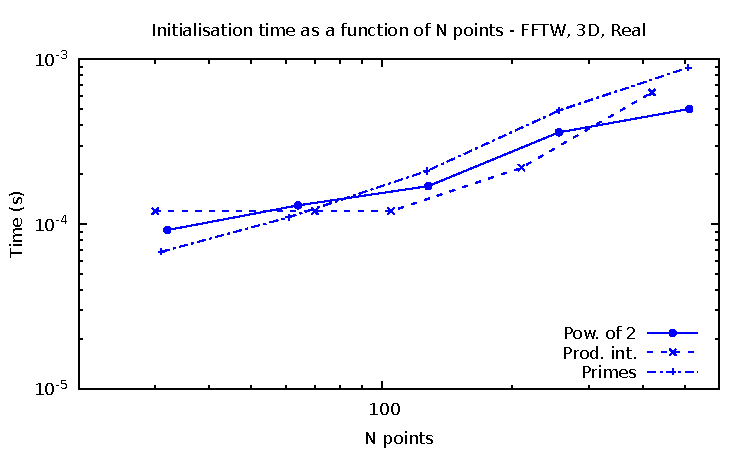
\includegraphics[width=.9\linewidth]{graphs/3d-fftw-init-r.pdf}
\caption{Intialisation (real)}
\label{3DFFTWRI}
\end{subfigure}%
\begin{subfigure}{.5\textwidth}
\centering
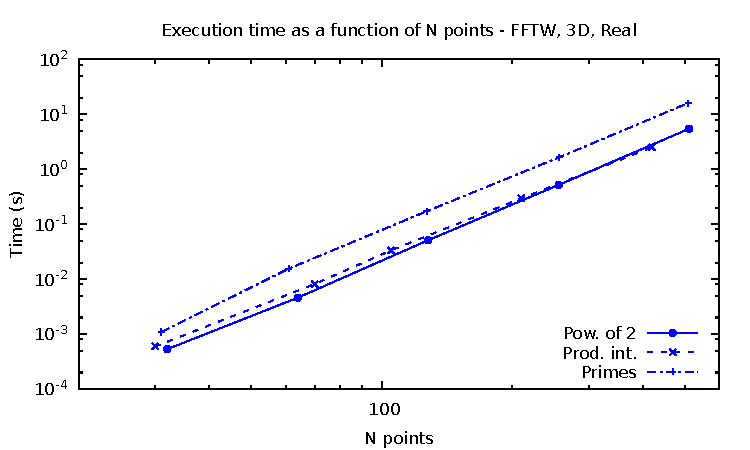
\includegraphics[width=.9\linewidth]{graphs/3d-fftw-exec-r.pdf}
\caption{Execution (real)}
\label{3DFFTWR}
\end{subfigure}\\
\begin{subfigure}{.5\textwidth}
\centering
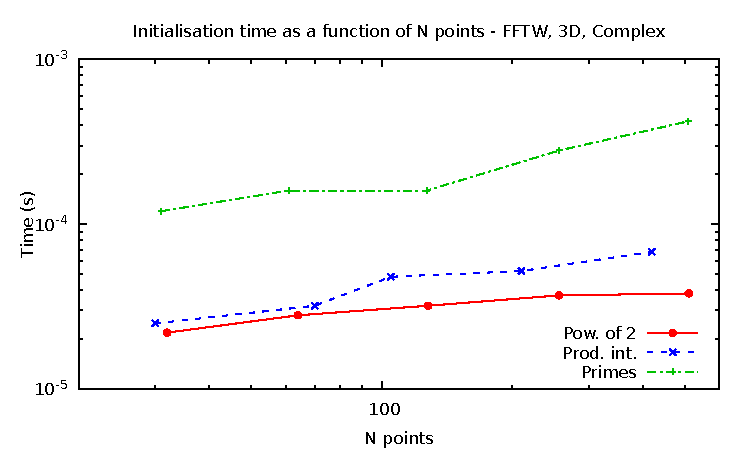
\includegraphics[width=.9\linewidth]{graphs/3d-fftw-init-c.pdf}
\caption{Intialisation (complex)}
\label{3DFFTWCI}
\end{subfigure}%
\begin{subfigure}{.5\textwidth}
\centering
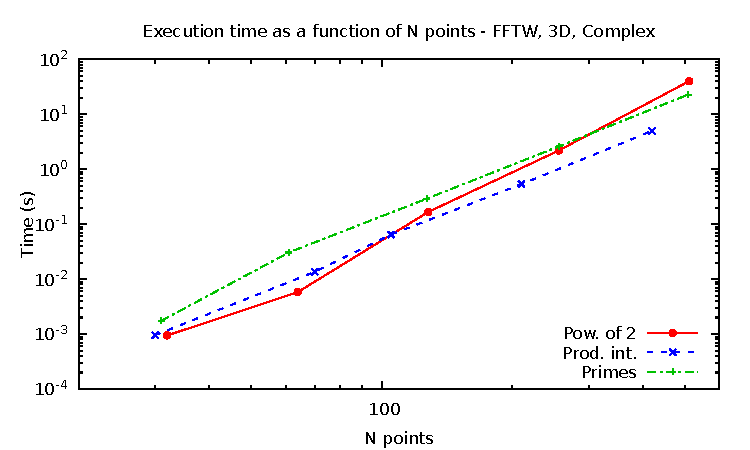
\includegraphics[width=.9\linewidth]{graphs/3d-fftw-exec-c.pdf}
\caption{Execution (complex)}
\label{3DFFTWC}
\end{subfigure}
\caption{Initialisation and execution times as a function of cube side (3 dimensions, FFTW, 1 thread)}
\label{3DFFTW}
\end{figure}


\begin{figure}[H]
\captionsetup{width=0.8\linewidth}
\centering
\begin{subfigure}{.5\textwidth}
\centering
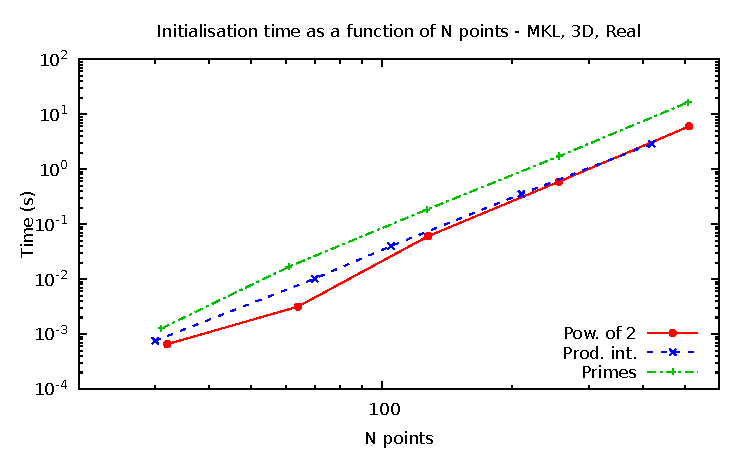
\includegraphics[width=.9\linewidth]{graphs/3d-mkl-init-r.pdf}
\caption{Intialisation (real)}
\label{3DMKLRI}
\end{subfigure}%
\begin{subfigure}{.5\textwidth}
\centering
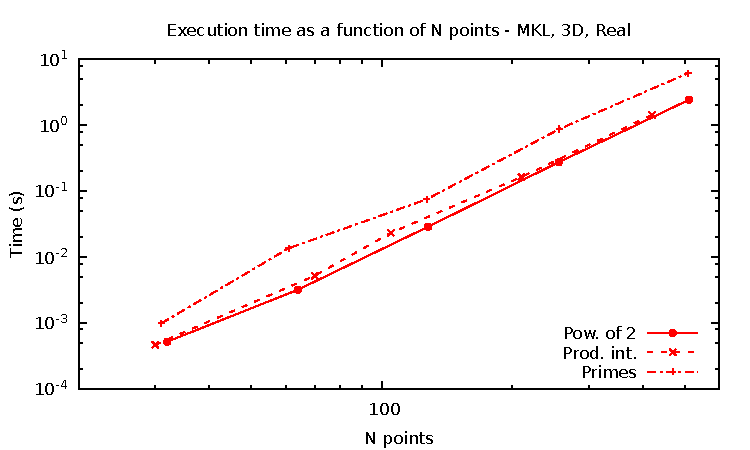
\includegraphics[width=.9\linewidth]{graphs/3d-mkl-exec-r.pdf}
\caption{Execution (real)}
\label{3DMKLR}
\end{subfigure}\\
\begin{subfigure}{.5\textwidth}
\centering
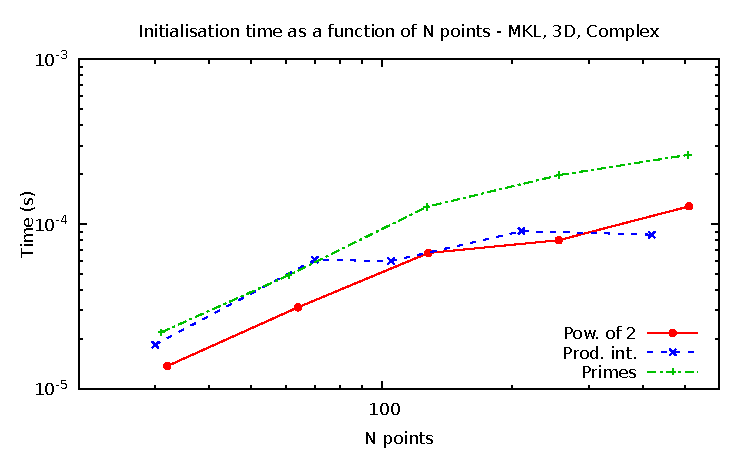
\includegraphics[width=.9\linewidth]{graphs/3d-mkl-init-c.pdf}
\caption{Intialisation (complex)}
\label{3DMKLCI}
\end{subfigure}%
\begin{subfigure}{.5\textwidth}
\centering
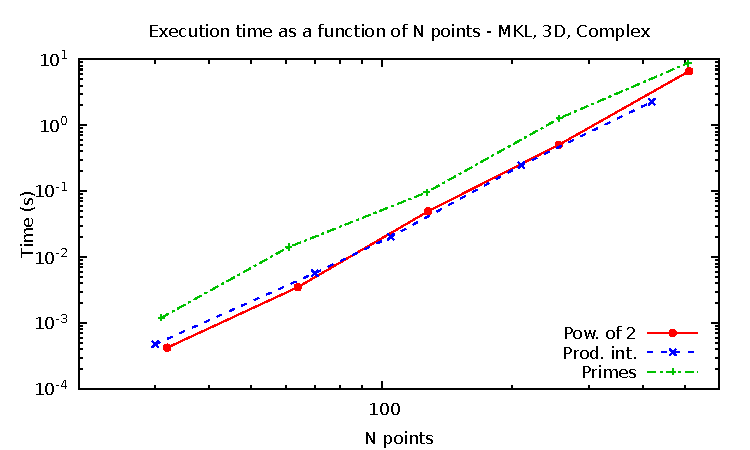
\includegraphics[width=.9\linewidth]{graphs/3d-mkl-exec-c.pdf}
\caption{Execution (complex)}
\label{3DMKLC}
\end{subfigure}
\caption{Initialisation and execution times as a function of cube side (3 dimensions, MKL, 1 thread)}
\label{3DMKL}
\end{figure}

\begin{figure}[H]
\captionsetup{width=0.8\linewidth}
\centering
\begin{subfigure}{.5\textwidth}
\centering
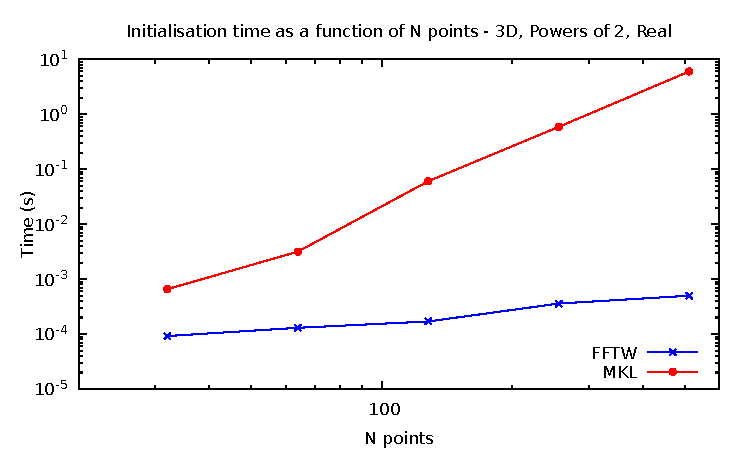
\includegraphics[width=.9\linewidth]{graphs/3d-pow2-init-r.pdf}
\caption{Intialisation (real)}
\label{3DPOW2RI}
\end{subfigure}%
\begin{subfigure}{.5\textwidth}
\centering
\includegraphics[width=.9\linewidth]{graphs/3d-pow2-exec-r.pdf}
\caption{Execution (real)}
\label{3DPOW2R}
\end{subfigure}\\
\begin{subfigure}{.5\textwidth}
\centering
\includegraphics[width=.9\linewidth]{graphs/3d-pow2-init-c.pdf}
\caption{Intialisation (complex)}
\label{3DPOW2CI}
\end{subfigure}%
\begin{subfigure}{.5\textwidth}
\centering
\includegraphics[width=.9\linewidth]{graphs/3d-pow2-exec-c.pdf}
\caption{Execution (complex)}
\label{3DPOW2C}
\end{subfigure}
\caption{Initialisation and execution times as a function of cube side (3 dimensions, powers of 2, 1 thread)}
\label{3DPOW2}
\end{figure}

\begin{figure}[H]
\captionsetup{width=0.8\linewidth}
\centering
\begin{subfigure}{.5\textwidth}
\centering
\includegraphics[width=.9\linewidth]{graphs/3d-init-r.pdf}
\caption{Intialisation (real)}
\label{3DRI}
\end{subfigure}%
\begin{subfigure}{.5\textwidth}
\centering
\includegraphics[width=.9\linewidth]{graphs/3d-exec-r.pdf}
\caption{Execution (real)}
\label{3DR}
\end{subfigure}\\
\begin{subfigure}{.5\textwidth}
\centering
\includegraphics[width=.9\linewidth]{graphs/3d-init-c.pdf}
\caption{Intialisation (complex)}
\label{3DCI}
\end{subfigure}%
\begin{subfigure}{.5\textwidth}
\centering
\includegraphics[width=.9\linewidth]{graphs/3d-exec-c.pdf}
\caption{Execution (complex)}
\label{3DC}
\end{subfigure}
\caption{Initialisation and execution times as a function of cube side\\(3 dimensions, 1 thread)}
\label{3D}
\end{figure}
\subsection{Effect of the flatness}\label{FLATNESS}

The experiments were carried out in Sections \ref{PERFORMANCE2D} and \ref{PERFORMANCE3D} where with domains whose dimensions were the same in all directions, that is, squares or cubes. In this section, we will study, in three dimensions, the effect of the flatness of the domain on the performance. We will compute the transform of a signal on a cuboid containing $512^3$ points stretched in the $z$ direction. The sides in the $x$ and $y$ directions have identical lengths ($N_x=N_y$) and the flatness is defined as the ratio between the number of points in the $z$ and $x$ directions ($N_z/N_x$). The dimensions of the domains considered appear in Table \ref{FLATNESSDIM}.
\begin{table}[H]
\centering
\begin{tabular}{|l|l|l|}
  \hline
  $N_x=N_y$ & $N_z $ & Flatness\\ 
  \hline
  \hline
512 & 512       & 1\\ \hline
256 & 2048      & 8\\ \hline
128 & 8192      & 64\\ \hline
64  & 32768     & 512\\ \hline
32  & 131072    & 4096\\ \hline
16  & 524288    & 32768\\ \hline
8   & 2097152   & 262144\\ \hline
4   & 8388608   & 2097152\\ \hline
2   & 33554432  & 16777216\\ \hline
1   & 134217728 & 134217728\\ \hline
\end{tabular}
\caption{Number of points used for the benchmark in three dimensions}\label{FLATNESSDIM}
\end{table}

We have observed that there is no clear trend in the way the flatness of the domain affects the performance and conclude that the performance depends mostly on the total number of points.\\
ngths, that is a square or a cube. 
\begin{figure}[H]
\captionsetup{width=0.8\linewidth}
\centering
\begin{subfigure}{.5\textwidth}
\centering
\includegraphics[width=.9\linewidth]{graphs/flatness-r.pdf}
\caption{Real}
\label{FLATNESSR}
\end{subfigure}%
\begin{subfigure}{.5\textwidth}
\centering
\includegraphics[width=.9\linewidth]{graphs/flatness-c.pdf}
\caption{Complex}
\label{FLATNESSC}
\end{subfigure}
\caption{Execution time as a function of the flatness of the domain ($N_y/N_x$), for $N_y=N_z$ (3 dimensions, powers of 2, 1 thread)}
\label{FLATNESS}
\end{figure}

\section{Parallelism}
So far, we have computed FFTs in a serial way. In this section, we will investigate the effect of parallelism on the performance achieved. Only the FFTW and MKL libraries are capable of taking advantage of the parallelism.  
\subsection{Multithreading}\label{MULTITHREADING}
We begin by considering the effect of multithreading on the computation of the transform of a cube of $512 \times 512 \times 512$ points. We carry out those measurements on a single node of ARCHER where we can use at most 24 threads. The MKL library is, once again, quicker. However FFTW scales a little better with the number of threads but it starts from  a lower performance.
\begin{figure}[H]
\captionsetup{width=0.8\linewidth}
\centering
\begin{subfigure}{.5\textwidth}
\centering
\includegraphics[width=.9\linewidth]{graphs/3d-multh-init-r.pdf}
\caption{Intialisation (real)}
\label{3DMULTHRI}
\end{subfigure}%
\begin{subfigure}{.5\textwidth}
\centering
\includegraphics[width=.9\linewidth]{graphs/3d-multh-exec-r.pdf}
\caption{Execution (real)}
\label{3DMULTHRE}
\end{subfigure}\\
\begin{subfigure}{.5\textwidth}
\centering
\includegraphics[width=.9\linewidth]{graphs/3d-multh-init-c.pdf}
\caption{Intialisation (complex)}
\label{3DMULTHCI}
\end{subfigure}%
\begin{subfigure}{.5\textwidth}
\centering
\includegraphics[width=.9\linewidth]{graphs/3d-multh-exec-c.pdf}
\caption{Execution (complex)}
\label{3DMULTHCR}
\end{subfigure}
\caption{Initialisation and execution times as a function of the number of threads (3 dimensions ($512 \times 512\times 512$ points), FFTW and MKL)}
\label{3DMKL}
\end{figure}

\subsection{MPI}\label{MPI}
We now turn to the studying the effect of the parallelism provided by MPI. In this case, we used up to 96 processes, corresponding to 4 ARCHER nodes, each with only a single thread. We carried out the measurements using a constant number of points on a line ($N_x=16777216$), a square ($N_x=N_y=4096$) and a cube ($N_x=N_y=N_z=256$). The MKL library is again more efficient, except in one dimension where it scales extremely poorly.
\begin{figure}[H]
\captionsetup{width=0.8\linewidth}
\centering
\begin{subfigure}{.5\textwidth}
\centering
\includegraphics[width=.9\linewidth]{graphs/mpi-init-1d.pdf}
\caption{Intialisation (real)}
\label{1DMPII}
\end{subfigure}%
\begin{subfigure}{.5\textwidth}
\centering
\includegraphics[width=.9\linewidth]{graphs/mpi-exec-1d.pdf}
\caption{Execution (real)}
\label{1DMPIE}
\end{subfigure}
\caption{Initialisation and execution times as a function of the number of processes (1 dimension)}
\label{1DMPI}
\end{figure}

\begin{figure}[H]
\captionsetup{width=0.8\linewidth}
\centering
\begin{subfigure}{.5\textwidth}
\centering
\includegraphics[width=.9\linewidth]{graphs/mpi-init-2d.pdf}
\caption{Intialisation (real)}
\label{2DMPII}
\end{subfigure}%
\begin{subfigure}{.5\textwidth}
\centering
\includegraphics[width=.9\linewidth]{graphs/mpi-exec-2d.pdf}
\caption{Execution (real)}
\label{2DMPIE}
\end{subfigure}
\caption{Initialisation and execution times as a function of the number of processes (2 dimensions)}
\label{2DMPI}
\end{figure}

\begin{figure}[H]
\captionsetup{width=0.8\linewidth}
\centering
\begin{subfigure}{.5\textwidth}
\centering
\includegraphics[width=.9\linewidth]{graphs/mpi-init-3d.pdf}
\caption{Intialisation (real)}
\label{3DMPII}
\end{subfigure}%
\begin{subfigure}{.5\textwidth}
\centering
\includegraphics[width=.9\linewidth]{graphs/mpi-exec-3d.pdf}
\caption{Execution (real)}
\label{3DMPIE}
\end{subfigure}
\caption{Initialisation and execution times as a function of the number of processes (3 dimensions)}
\label{3DMPI}
\end{figure}

\subsection{MPI and multithreading}\label{MPIMULTH}
We now combine multithreading with MPI in the same consitions as in Section \ref{MPI}. We increase the number of threads up to the number of cores on a compute node and subsequently increase the number of such processes. We carry out this procedure till we use 4 processes, each consisting of 24 threads. In two dimensions, the performance is better with the MKL. However, once we use MPI, the scaling provided by multithreading becomes really poor. In one dimension, the MKL scales poorly and FFTW turns out to yield a higher performance. Finally, in three dimensions, FFTW crashes and the MKL runs only on a single node. 
\begin{figure}[H]
\captionsetup{width=0.8\linewidth}
\centering
\begin{subfigure}{.5\textwidth}
\centering
\includegraphics[width=.9\linewidth]{graphs/mpi-multh-init-1d.pdf}
\caption{Intialisation}
\label{1DMPIMULTHI}
\end{subfigure}%
\begin{subfigure}{.5\textwidth}
\centering
\includegraphics[width=.9\linewidth]{graphs/mpi-multh-exec-1d.pdf}
\caption{Execution}
\label{1DMPIMULTHE}
\end{subfigure}
\caption{Initialisation and execution times as a function of the number of cores (1 dimension)}
\label{1DMPIMULTH}
\end{figure}

\begin{figure}[H]
\captionsetup{width=0.8\linewidth}
\centering
\begin{subfigure}{.5\textwidth}
\centering
\includegraphics[width=.9\linewidth]{graphs/mpi-multh-init-2d.pdf}
\caption{Intialisation}
\label{2DMPIMULTHI}
\end{subfigure}%
\begin{subfigure}{.5\textwidth}
\centering
\includegraphics[width=.9\linewidth]{graphs/mpi-multh-exec-2d.pdf}
\caption{Execution}
\label{2DMPIMULTHE}
\end{subfigure}
\caption{Initialisation and execution times as a function of the number of cores (2 dimensions)}
\label{2DMPIMULTH}
\end{figure}

\begin{figure}[H]
\captionsetup{width=0.8\linewidth}
\centering
\begin{subfigure}{.5\textwidth}
\centering
\includegraphics[width=.9\linewidth]{graphs/mpi-multh-init-3d.pdf}
\caption{Intialisation}
\label{3DMPIMULTHI}
\end{subfigure}%
\begin{subfigure}{.5\textwidth}
\centering
\includegraphics[width=.9\linewidth]{graphs/mpi-multh-exec-3d.pdf}
\caption{Execution}
\label{3DMPIMULTHE}
\end{subfigure}
\caption{Initialisation and execution times as a function of the number of cores (3 dimensions)}
\label{3DMPIMULTH}
\end{figure}

\subsection{Constant number of cores}\label{CONST}
We now compare the effects of multithreading and MPI by using a constant number of cores, 24, on a single node while varying the number of processes and threads. The signal is the same as in Sections \ref{MPI} and \ref{MPIMULTH}. We reach the same conclusions as previously. Unlike what happens with a single process (Section \ref{MULTITHREADING}), when combibed with MPI, does not seem to yield a significan performance improvement. As a consequence, the performance improves only with an increasing number of threads. In two dimensions, the best performance is achieved with the MKL. However, in one dimension, FFTW scales better and is more efficient with a larger number of processes. In three dimensions, we have only obtained data with the MKL library since FFTW crashes.
\begin{figure}[H]
\captionsetup{width=0.8\linewidth}
\centering
\begin{subfigure}{.5\textwidth}
\centering
\includegraphics[width=.9\linewidth]{graphs/const-init-1d.pdf}
\caption{Intialisation}
\label{1DCONSTI}
\end{subfigure}%
\begin{subfigure}{.5\textwidth}
\centering
\includegraphics[width=.9\linewidth]{graphs/const-exec-1d.pdf}
\caption{Execution}
\label{1DCONSTE}
\end{subfigure}
\caption{Initialisation and execution times as a function of the number of processes (1 dimension)}
\label{1DCONST}
\end{figure}

\begin{figure}[H]
\captionsetup{width=0.8\linewidth}
\centering
\begin{subfigure}{.5\textwidth}
\centering
\includegraphics[width=.9\linewidth]{graphs/const-init-2d.pdf}
\caption{Intialisation}
\label{2DCONSTI}
\end{subfigure}%
\begin{subfigure}{.5\textwidth}
\centering
\includegraphics[width=.9\linewidth]{graphs/const-exec-2d.pdf}
\caption{Execution}
\label{2DCONSTE}
\end{subfigure}
\caption{Initialisation and execution times as a function of the number of processes (2 dimensions)}
\label{2DCONST}
\end{figure}

\begin{figure}[H]
\captionsetup{width=0.8\linewidth}
\centering
\begin{subfigure}{.5\textwidth}
\centering
\includegraphics[width=.9\linewidth]{graphs/const-init-3d.pdf}
\caption{Intialisation}
\label{3DCONSTI}
\end{subfigure}%
\begin{subfigure}{.5\textwidth}
\centering
\includegraphics[width=.9\linewidth]{graphs/const-exec-3d.pdf}
\caption{Execution}
\label{3DCONSTE}
\end{subfigure}
\caption{Initialisation and execution times as a function of the number of processes (3 dimensions)}
\label{3DCONST}
\end{figure}


\section{Requirements from the CCP}\label{CCPPETMR}
We have also benchmarked the FFT libraries in a situation corresponding to a problem encountered by the CCP/PET-MR collaboration, by computing the transform of a series of 32 square complex images whose side consists of 256 points as well as the closest prime number (257) and product of powers of small integers ($2^23^27=252$). We have repeated the algortihm described in Table \ref{PSEUDOCODE} but, this time, with $N_{SIGNALS}=32$. As in the other cases, the MKL library performs better than FFTW. None of the other libraries we have considered could be used in this situation. GSL works only in one dimension. The FORTRAN version of FFTPACK does not share that limitation. However all the C/C++ wrappers we have found offer only one-dimensional transforms. Finally FFTPACK is distributed with a licence that is less constraining than the GPL but, nevertheless, the C++ wrapper provided by CASA that we have used is distributed under the GPL v2.

\begin{figure}[H]
\captionsetup{width=0.6\textwidth}
\centering
\includegraphics[height=8cm]{graphs/ccppetmr.pdf}
\caption{Execution time for the transform of 32 complex square images as a function of square side\\(2 dimensions, complex, 1 thread)}
\label{method}
\end{figure}
\section{Conclusion}
In our experiments, the MKL library tended to perform better. Things are less clear in a single dimension. However, even in that case, it remains among the best, especially with real numbers, in more challenging circumstances, when the number of points in large and consists in the product of small integers or a prime number.  
\section{Acknowledgements}
The special sentence that only Barbara knows.
\begin{thebibliography}{9}

\bibitem{CT}
Cooley J. W., Tukey J. W.
{\it An algorithm for the machine calculation of complex Fourier series},
Math. Comp. 19 (1965), 297-301
 
\bibitem{fftw}
Frigo, Matteo and Johnson, Steven G.,
{\it The Design and Implementation of FFTW3},
Proceedings of the IEEE,
2005,
93,
2,
216--231,
Special issue on ``Program Generation, Optimization, and Platform Adaptation''
\bibitem{mkl}
\hyperlink{https://software.intel.com/en-us/mkl}{https://software.intel.com/en-us/mkl}

\bibitem{gsl}
M. Galassi et al, {\it GNU Scientific Library Reference Manual (3rd Ed.)}, ISBN 0954612078
  
\bibitem{fftpack}
P.N. Swarztrauber, {\it Vectorizing the FFTs}, Parallel Computations (G. Rodrigue, ed.), Academic Press, 1982, pp. 51--83.
  
\bibitem{casa}
McMullin J. P., Waters B., Schiebel D., Young W., Golap K.,
{\it Astronomical Data Analysis Software and Systems XVI},
ASP Conf. Ser. 376, ed. R. A. Shaw, F. Hill, D. J. Bell (San Francisco, CA: ASP), 127

\bibitem{code}
\hyperlink{git@github.com:SoftwareOutlook/FFTC.git}{git@github.com:SoftwareOutlook/FFTC.git}
    
\bibitem{ccppetmr}
\hyperlink{https://www.ccppetmr.ac.uk/}{https://www.ccppetmr.ac.uk/}

\bibitem{softwareoutlook}
\hyperlink{https://www.softwareoutlook.ac.uk/}{https://www.softwareoutlook.ac.uk/}

\bibitem{archer}
ARCHER: UK National Computing Service, \hyperlink{https://www.archer.ac.uk/}{https://www.archer.ac.uk/}
  
\end{thebibliography}

\end{document}
